\documentclass[a4paper]{article}

\usepackage[utf8]{inputenc}   % LaTeX, comprends les accents !
\usepackage[T1]{fontenc}      % Police contenant les caractères français
\usepackage[french]{babel}  
\usepackage{fullpage}
\usepackage{graphicx}
\usepackage{wrapfig}
\usepackage{float}
\usepackage{blindtext}
\usepackage{algorithm2e}
% \usepackage[open,openlevel=1]{bookmark}
\usepackage[colorlinks=true,linkcolor=black,urlcolor=black,bookmarksopen=true,bookmarksnumbered=true]{hyperref}
\usepackage{bookmark}
\usepackage{blindtext}
% \usepackage{biblatex}

\RestyleAlgo{ruled}
\graphicspath{ {./img/} }

\begin{document}
	\title{Reconnaissance de l'écriture manuscrite\\Rapport de projet}
	\author{Laurent Antoinette, Romain Campillo, Tony Nguyen\\\emph{L3 informatique}\\
	Faculté des Sciences\\
	Université de Montpellier.}
	\date{\today}
	\maketitle
	\thispagestyle{empty}
	\begin{figure}[h]
		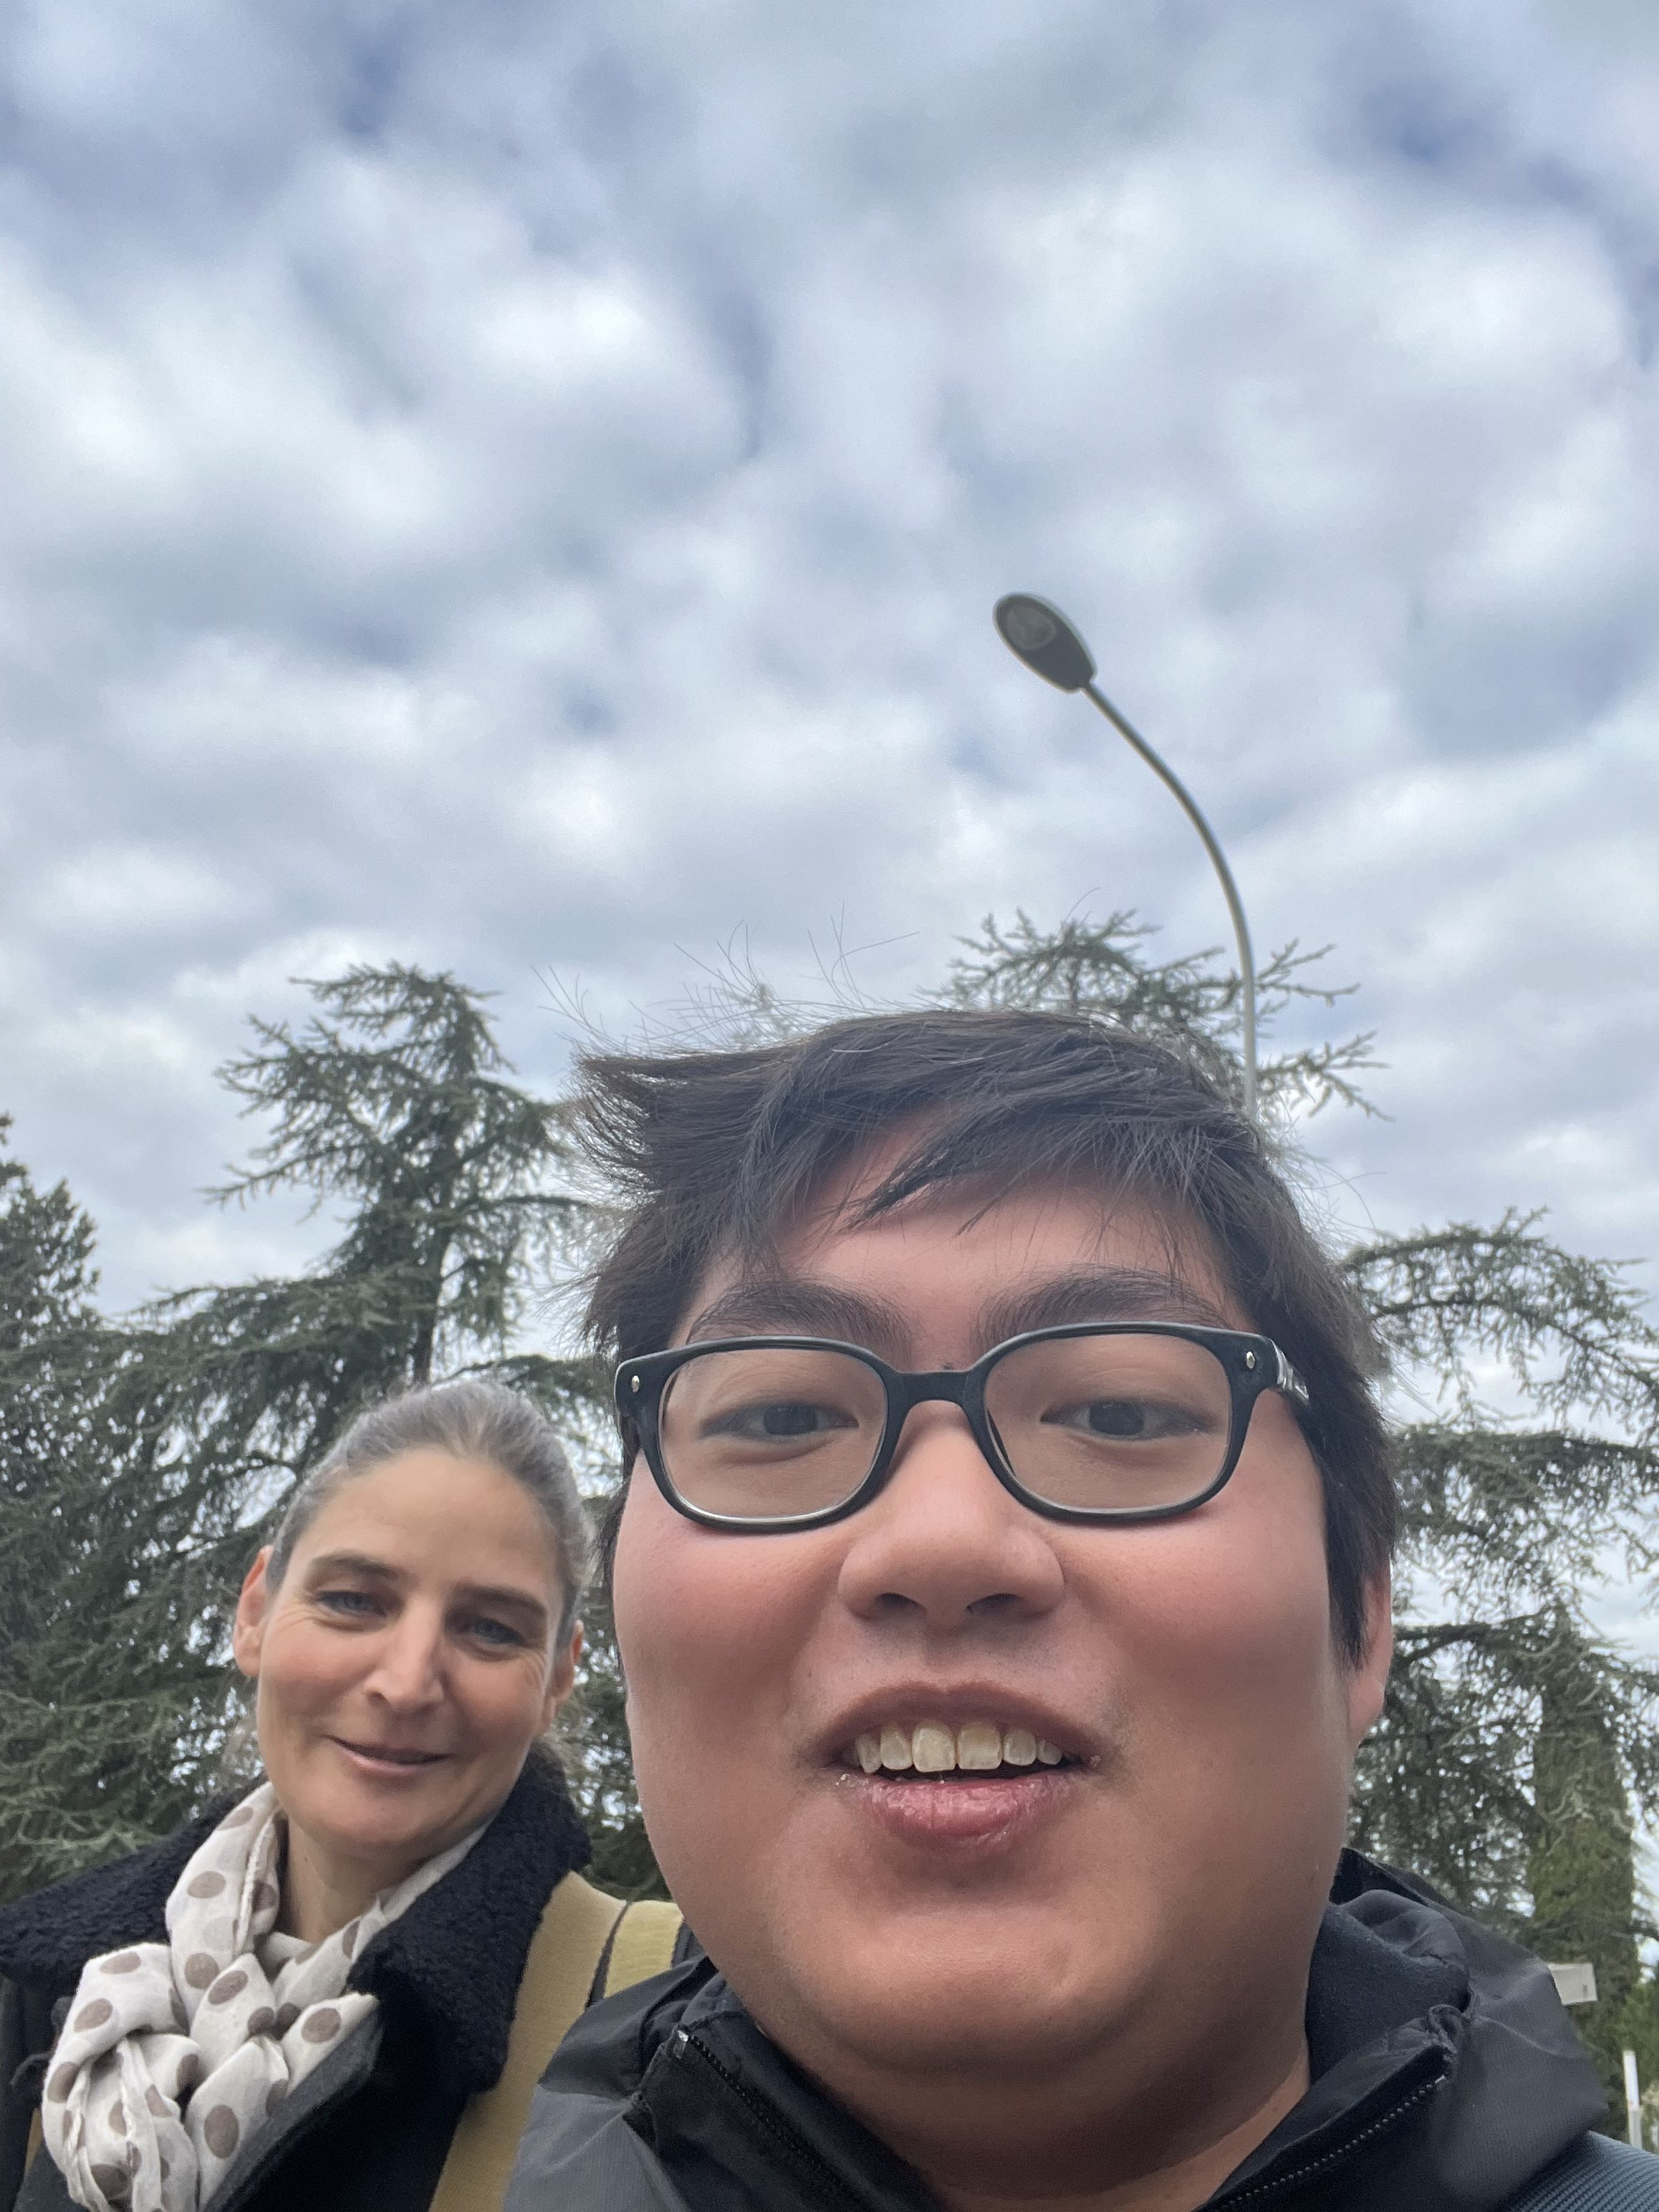
\includegraphics[scale=.1]{selfie_tony_clementine.jpg}
		% 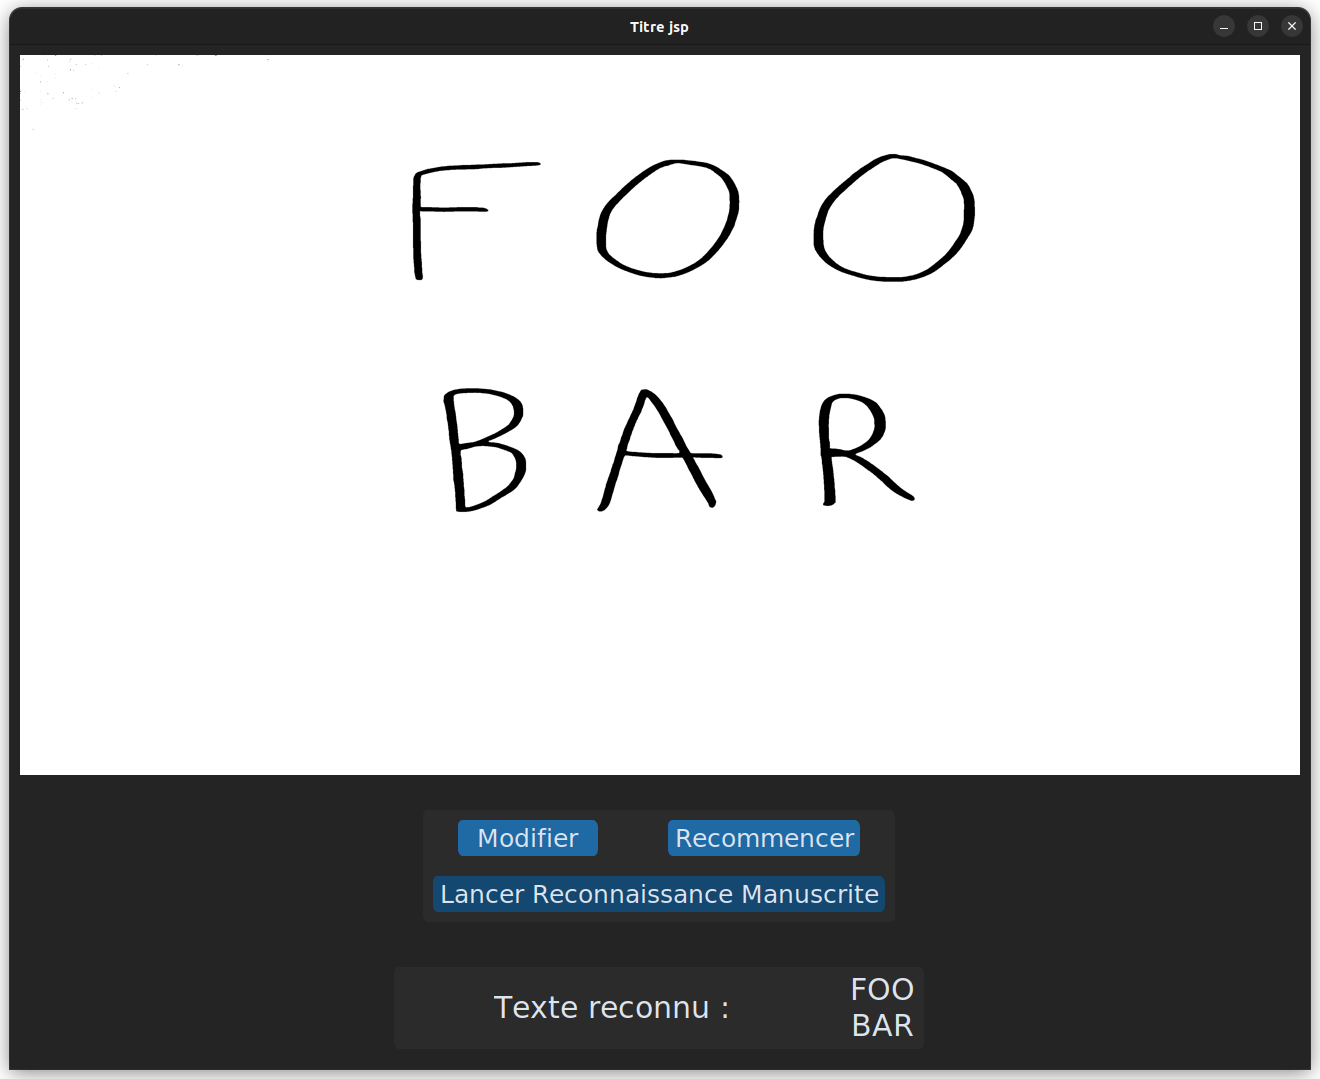
\includegraphics[width=\textwidth]{recon.png}
		\centering
	\end{figure}
	\newpage
	\thispagestyle{empty}
	\tableofcontents
	\newpage
	\thispagestyle{empty}
	\listoffigures
	\listofalgorithms
	\newpage
	\section{Présentation du Sujet } 
		\subsection{La problématique}
			\paragraph{}
				La reconnaissance de l'écriture manuscrite consiste à traduire un texte manuscrit en un texte numérique, interprétable par l'ordinateur. Bien que cette application commence à être utilisé dans différents secteurs, 
				la variation des styles d'écritures manuscrites d'une personne à l'autre et la mauvaise qualité du texte pose des défis importants pour leurs numérisations.% manuscrits en texte numérique.%  convertion en texte numérique.
\\Les méthodes classiques étudiées auparavant ou présentées dans la littérature, notamment l'amélioration de la qualité d'images (filtres, etc) ou la reconnaissance des formes complexes, peuvent ne pas répondre à ce type de problématique.
\\Ainsi dans ce projet, nous allons explorer un autre axe de recherche basée sur les méthodes de réseaux de neuronne qui ont prouvé leur efficacité à reconnaître et classifier les formes les plus complexes.
\\Cette recherche va nous permettre de mettre en oeuvre nos compétences en traitement d'image et d'explorer de nouvelles méthodes plus avancées.

			% L'essence du problème est qu'un texte dans un document est très diffrent d'une photo du même document. Dans le 1er cas, le format rend le contenu comprehensible par un ordinateur, il peut donc 
			% chercher un mot dans le texte ou le modifier pour corriger des fautes d'orthographe. Dans le 2e cas, l'image représente la même chose. MAIS, la machine ne comprend le sens de l'information 
			% représentée. Il voit les pixels mais pas les charactères. De plus, des imperfections dans la capture du document changent la photo (ex: luminosité, angle ...), il y a une modification des informations
			% alors que le texte ne change pas.
			% \\Réussir à lire du texte sur des images permettrait de faciliter la numérisation de document papier. Ainsi, libérer les Humains de quelques tâches redondantes. Lire des formulaires ou encore d'améliorer les moteurs de recherche avec des images qui contient du texte sont des applications possibles.
		\subsection*{}
			Le traitement automatique de l'information numérique est particulièrement intéressant compte tenu des enjeux actuels. Notamment, vis à vis du développement des IAs étant très utilisées par les entreprises 
			sachant le gain de temps et de productivité considérable que ces dernières peuvent leurs apporter.

			%pour des étudiants en informatique car il peut être abordé de nombreuses manières. 

			% L'utilisation de l'intelligence artificielle et notamment des réseaux de neurones permettrait de reconnaitre facilement les formes
			% Grâce à la croissance exponentielle de l'intelligence artificielle ces dernières années,
			% nous pouvons 
			%  En effet, un projet sur le traitement automatique de l'information numérique est exactement ce que des étudiants en informatique devraient faire. Nous avons pu constater une explosion
			% de l'intelligence artificielle ces dernières années, notamment les réseaux neuronaux. À l'heure actuelle, ils sont capables de détecter des objets et de les classifier. Ce projet est tout à fait 
			% intéressant pour de futurs étudiants en master IASD.
		\subsection{Quelques approches de reconnaissance de formes}
			\subsubsection{k-Nearest Neighbor}
				La méthode du k-Nearest Neighbor se base sur le principe que les échantillons appartenant à la même classe ont tendance à se regrouper dans l'espace des caractéristiques.
				Pour classifier une nouvelle entrée, on regarde les k points d'entraînement les plus proches. La nouvelle entrée est classée en fonction de la classe majoritaire des voisins
				% Méthode statistique, il y a un plan avec plein d'objets qui forment des troupeaux, notre lettre est quelque part dans le plan, on trace un cercle autour, notre lettre est identifiée comme l'objet présent au plus grand nombre à l'intérieur du cercle.
			\subsubsection{Template matching} 
				% En gros, comparaison de l'image avec la base de donnée entière à l'aide d'une fonction de distance. 
				\paragraph{}
					Cette approche est l'une des plus simple. Voici en quoi elle consiste :\\Nous allons partir d'une banque d'image de référence. Puis lorsqu'une nouvelle image devra être classifiée, une simple comparaison entre cette image et les images de référence sera faite à l'aide d'une fonction de distance euclidienne.
				\paragraph{} L'avantage de cette solution est qu'il n'est pas nécessaire d'entrainer un modèle au préalable. Elle est néanmoins sensible aux rotations et aux déplacements dans l'image.%si la nouvelle image subit une rotation trop grande,
			\subsubsection{Les réseaux de neuronnes} 
				Les réseaux de neuronnes sont souvent utilisés pour résoudre des problèmes de classification et de prédiction.
				Ils sont constitués de couches de neurones interconnectées en s'inspirant du fonctionnement du cerveau humain.
				Cette méthode nécessite une phase d'apprentissage qui peut être longue, coûteuse et qui repose sur la qualité et la quantité des données d'entraînement fournies.
				\\Nous avons choisi cette solution pour procéder à la reconnaissance des caractères dans notre projet.

		\subsection{Cahier des charges}

			\subsubsection{Objectifs}
			Notre objectif est de proposer une méthode pour convertir une image de texte manuscrit en un texte numérique.\\
			Dans notre étude nous allons considérer les 26 lettres de l'alphabet latin en majuscule et espacées.


			\subsubsection{Besoins et contraintes}
				\paragraph{Les besoins}
					\subparagraph{Capturer une image}
						L'utilisateur pourra prendre des photos par notre logiciel à l'aide d'une webcam. Mais il pourra également importer des images depuis son système de fichier. Tout cela à travers une interface Homme-Machine.
					\subparagraph{Pré-traitement}
						Le logiciel devra améliorer la qualité de l'image capturée en appliquant une réduction bruit et l'utilisation de filtres prédéfinis. 
					\subparagraph{Segmentation de l'image}
						Les différents caractères présents sur l'image seront localisés à l'aide de la projection verticale et horizontale de l'histogramme.
					\subparagraph{Extraction des caractères}
						Chaque caractère présent dans l'image d'entrée sera extrait sous forme d'imagette à l'aide des coordonnées calculées dans la partie segmentation.  
					\subparagraph{Reconnaissance}
						Les caractères, étant sous formes d'imagettes, feront l'objet d'une reconnaissance de façon individuelle grâce à un réseau neuronal convolutif.  
					\subparagraph{Présenter}
						Une fois les caractères manuscrits reconnus en caractères numériques. Ils seront assemblés, puis affichés à l'utilisateur.
				\paragraph{Les contraintes}
					Nous nous fixons comme contraintes de ne pas utiliser de services comme Google Collab car Google possède un modèle économique type "Freemium" (initialement gratuit mais avec des fonctinalités payantes). Nous souhaitons créer un logiciel suffisament performant pour qu'il puisse être lancé sur l'une de nos machines personelles. \\De plus, une webcam est nécessaire, ou alors un appareil photo numérique.
			\subsubsection{Résulats attendus}
				\paragraph{}
					Notre programme doit reconnaître des lettres manuscrites sur un fond blanc. Les lettres seront des caractères majuscules non-liés et sans accents ni caractères spécials.
	\section{Technologies utilisées} 
		\subsection{Langages et outils}
			\subsubsection{Python3}
				Python3 est un langage de programmation interprété, multiparadigme et multiplatforme. Il favorise la programmation impérative structurée, fonctionnelle et orientée objet. Il est doté d'un typage dynamique fort, d'une gestion automatique de la mémoire par ramasse-miettes et d'un système de gestion d'exceptions. (\url{https://fr.wikipedia.org/wiki/Python_(langage)})

				% Test \cite{textbook}
				% \cite{web:lang:python}
			\subsubsection{OpenCV}
				\begin{wrapfigure}{r}{0.15\textwidth}
					
\includegraphics[width=0.15\textwidth]{OpenCV.png}
				\end{wrapfigure}
				OpenCV (Open Computer Vision) est une bibliothèque open source spécialisée dans le traitement d'images en temps réel.
				Elle est déposée sous licence libre, et sa popularité ainsi que sa simplicité d'utilisation en font un outil adéquat pour notre projet.
				Parmi ses nombreuses fonctionnalités, nous utiliserons surtout ses fonctions de filtrage et de seuillage.
				
				\newline
			\subsubsection{You Only Look Once}
				\paragraph{}
				You Only Look Once (YOLO) est une archicture de Réseau Neuronal Convolutif (CNN) de type "Region based" (R-CNN) qui est capable de localiser des objets dans une image et, en même temps, de les classifier.

				\paragraph{Les réseaux de neurones}
					Les réseaux de neurone simulent plus ou moins le fonctionnement du cerveau humain. Ils sont constitués d'une multitude de neurones interconnectés entre eux qui reçoivent et renvoient des informations.
					\subparagraph{} Un neurone prend plusieurs entrées pondérées, les somme, puis les passe à travers une fonction d'activation pour produire une sortie vers un autre neurone.
					\subparagraph{} L'architecture des réseaux de neurone simple est organisée en couche. La 1ère couche représente l'entrée et la dernière couche la sortie.
					Entre le début et la fin du réseau, les couches intermédiaires sont connectées vers l'avant et de façon complète. Un neurone est connecté à tous les neurones de la couche précédente et de la suivante mais pas à ceux de la même couche.
					L'apprentissage d'un réseau de neurones en couches se fait par rétropropagation, où l'erreur entre la sortie du réseau et la sortie attendue est propagée en arrière dans le réseau, et les poids des connexions entre les neurones sont ajustés pour minimiser cette erreur.
					Ce processus est répété pour chaque exemple d'entraînement jusqu'à ce que le réseau atteigne un niveau de précision satisfaisant.	
						
					\subparagraph{Les Réseaux de Neurones Convolutifs (CNN)} 
					Contrairement aux réseaux de neurones traditionnels, qui utilisent des connexions denses entre les neurones des couches adjacentes, les CNN utilisent des couches de convolution qui appliquent des filtres pour extraire des caractéristiques importantes de l'image.
					Cette opération permet d'extraire des motifs et des formes à différentes échelles et positions de l'image.
					Les couches de sortie du CNN sont des couches denses classiques qui combinent les informations extraites par les couches précédentes pour produire une sortie finale, telle que la classe de l'objet présent dans l'image.
					\subparagraph{Region Based CNN}


					\subparagraph{} YOLO 

		\subsection*{Justification}
			\subsubsection*{Python3}
				\paragraph{} Nous avons choisi ce langage car il est simple à comprendre et relativement facile à lire. De plus, par sa popularité, il existe de nombreuses bibliothèques dont les fonctions répondent à nos besoins. Python étant conçu pour faciliter la programmation, nous pourrons nous concentrer davantage sur le développement de nos algorithmes et être efficace quant à leur implementation.
			\subsubsection*{OpenCV}
				\paragraph{} Effectivement, cette bibliothèque dispose de nombreuse fonction qui nous sont utiles. De plus, elle est populaire, sous licence libre et développé par Intel.
			\subsubsection*{You Only Look Once}
				\paragraph{} YOLO est un réseau de neuronne convolutif moderne est performant implément de nombreuses innovation des dernières années.
	\newpage
	\section{Développements Logiciel : Conception, Modélisation, Implémentation}
		\begin{figure}[h]
			\caption{Diagramme de cas d'utilisation}
			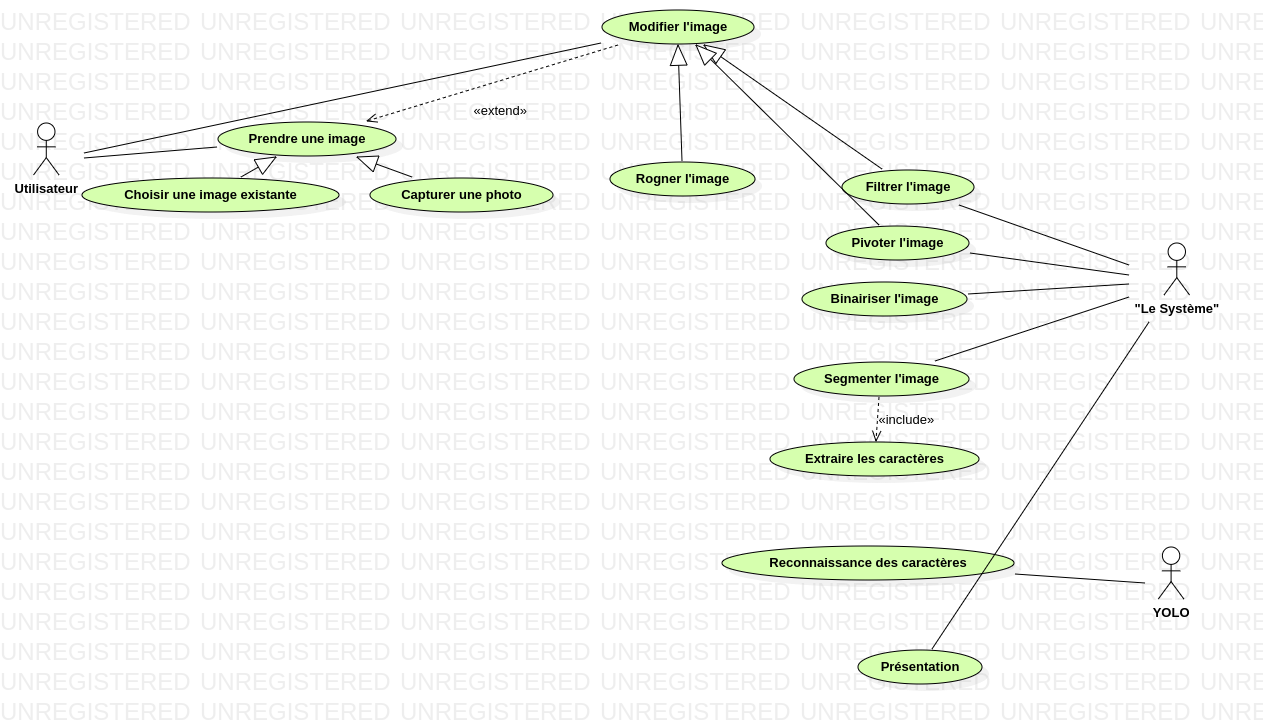
\includegraphics[width=\textwidth]{UseCaseDiagram.png}
			\centering
			\label{fig:useCaseDiagram}
		\end{figure}
		\subsection{Interface Homme-Machine}
			L'IHM nous permet de prendre des photos avec une webcam connectée à l'ordinateur ou choisir à partir d'une fenêtre une image déjà existante. 
%Diagramme de Cas d'Utilisation à la page \pageref{fig:useCaseDiagram}. 
			\begin{figure}[H]
				\caption{Fenêtre de l'IHM où l'on peut rogner, pivoter et filtrer une image}
				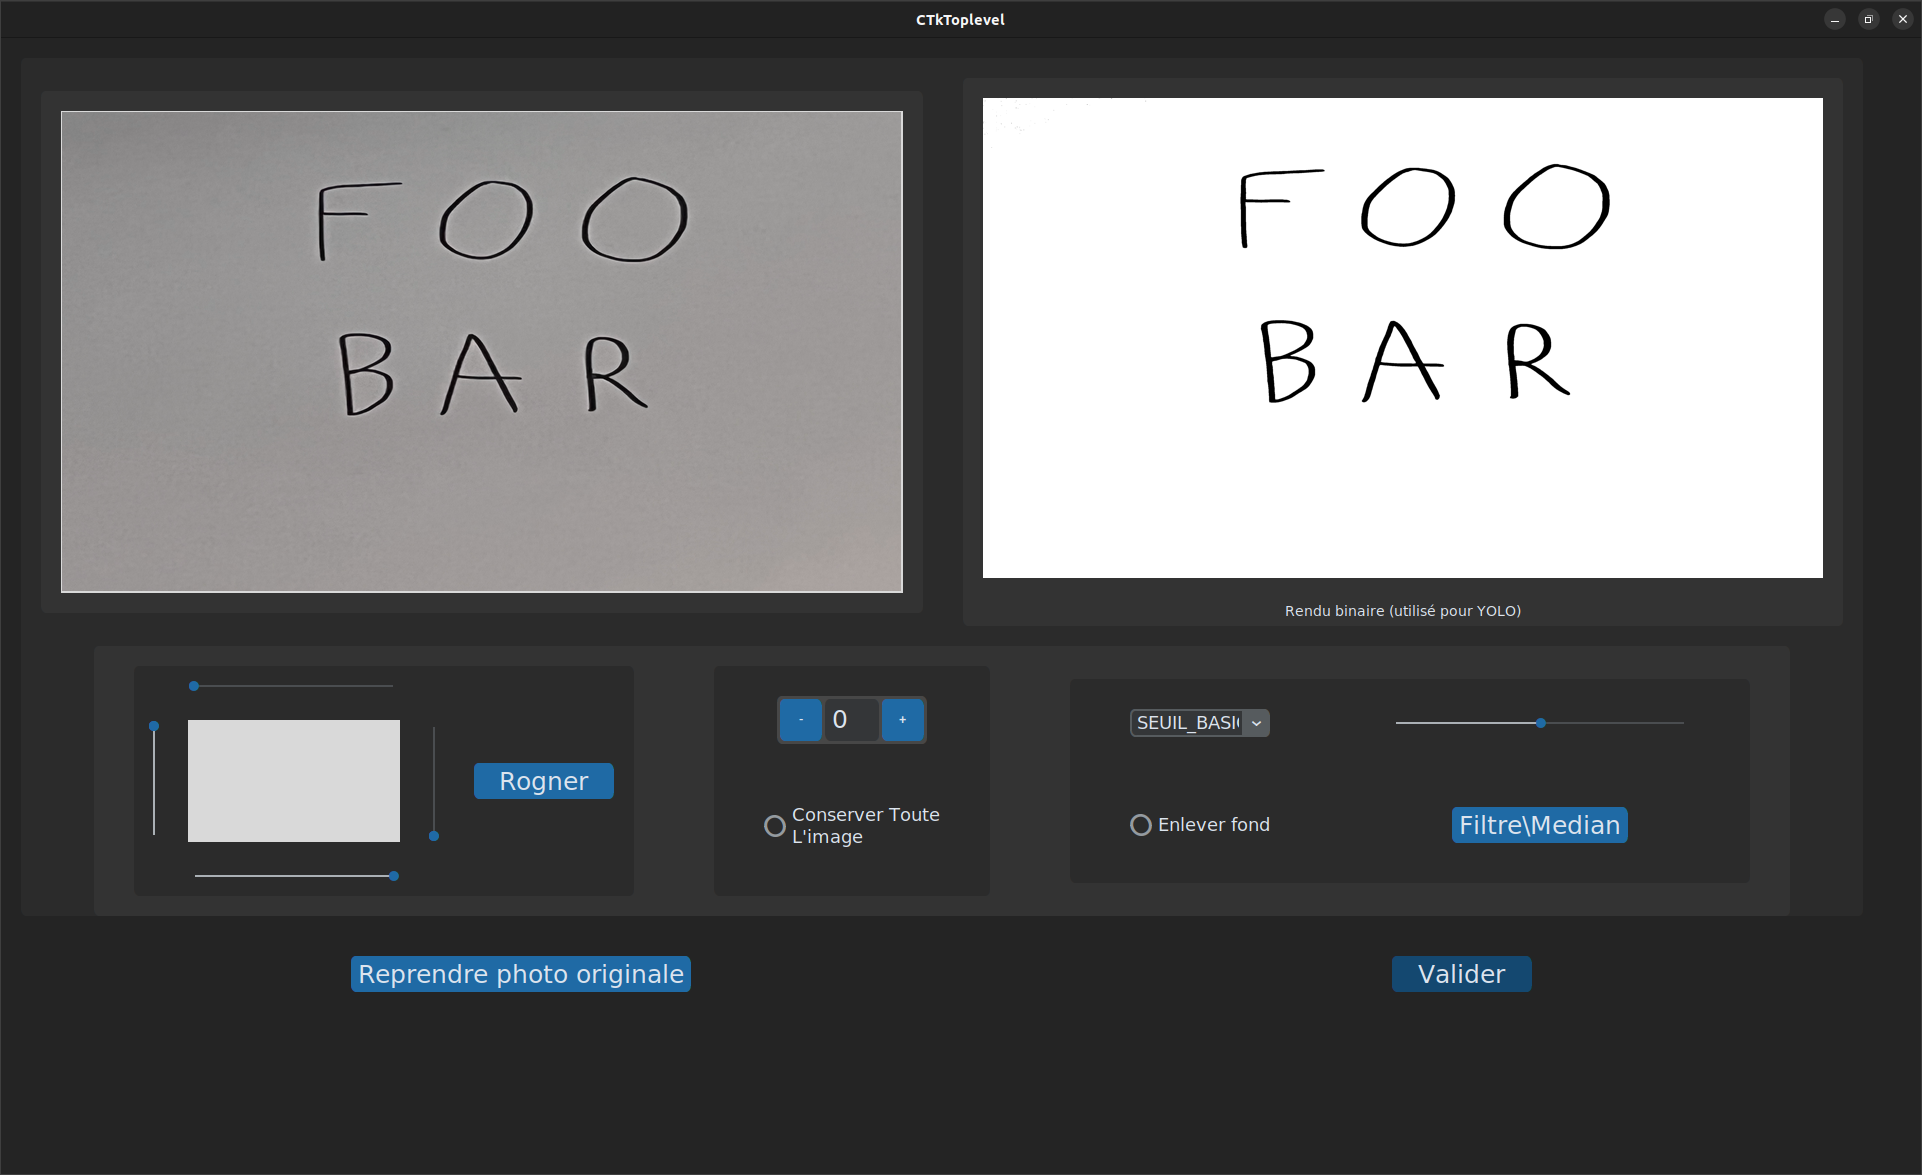
\includegraphics[width=0.8\textwidth]{modif.png}
				\centering
				\label{fig:modif}
			\end{figure}
			\paragraph{}
				Après avoir entrer une image (figure 2 A), une étape de préprocessing (découpage) peut-être établi pour réduire le bruit concentrer sur les bords de l'image et causé par la lumière .
				L'image résultat est convertie après en image binaire réalisé avec un seuil adapté. Puis, les pixels noirs et blancs ont été inversé pour facilité la segmentation des images.
				%il est possible qu'il y ait beaucoup de bruit, dans ce cas là, nous pouvons rogner l'image pour enlever des ombres sur les bords, faire des rotations et filtrer pour enlever le bruit comme illustrée sur la figure \ref{fig:modif}
			\begin{figure}[H]
				\caption{Fenêtre de l'IHM après présentation des caractères reconnus}
				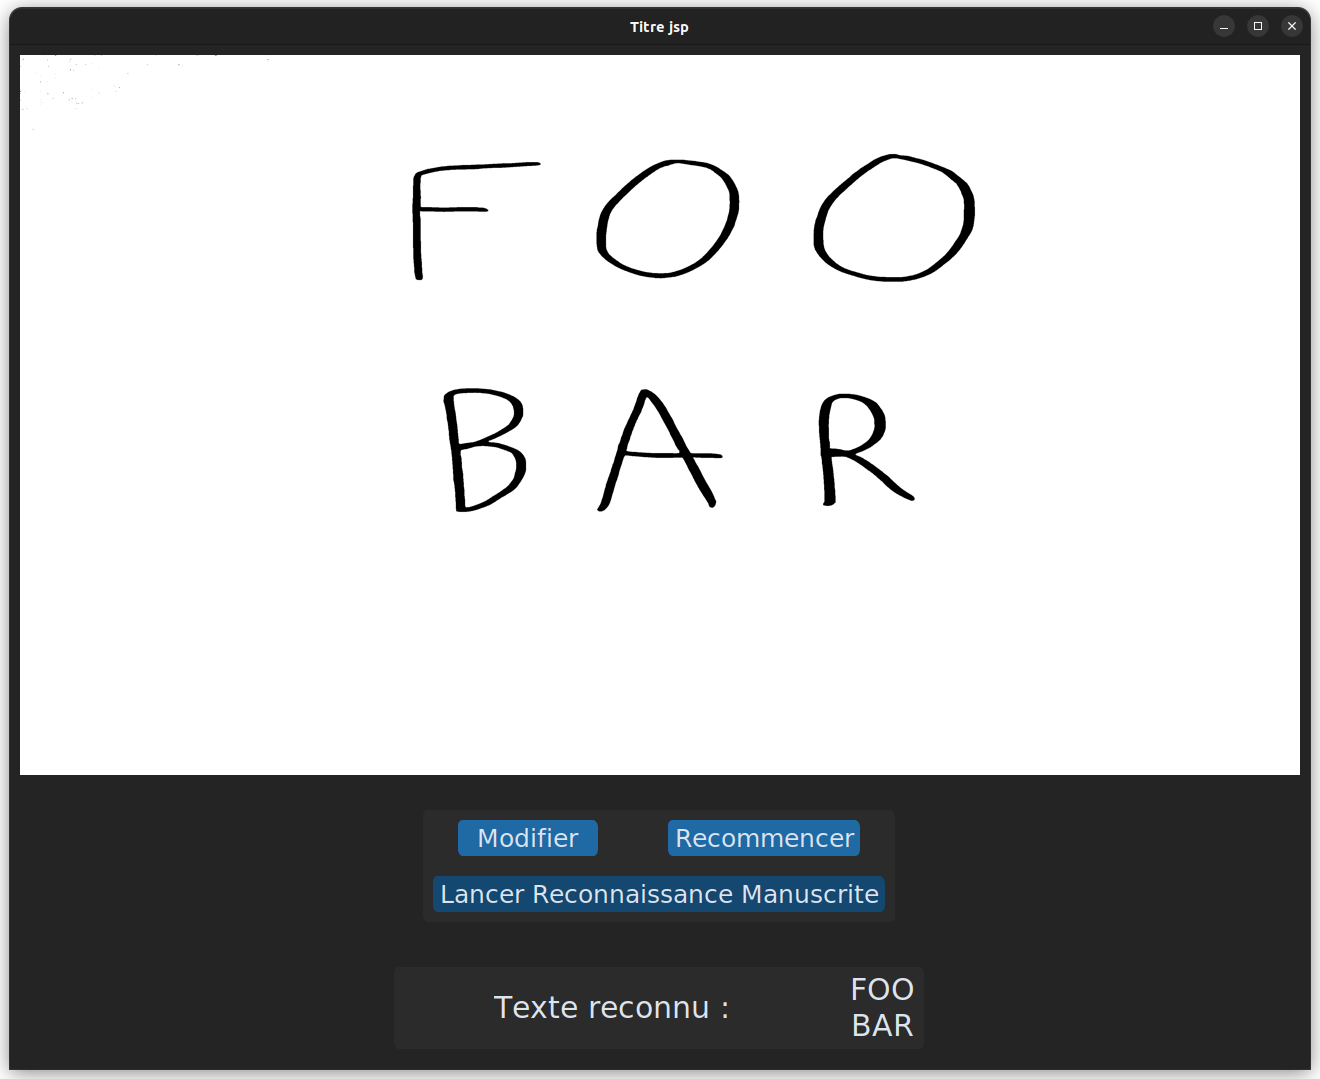
\includegraphics[width=0.8\textwidth]{recon.png}
				\centering
				\label{fig:recon}
			\end{figure}
			\paragraph{} Après avoir établi le prétraitement détaillé ci-dessus, on va procéder à la segmentation des caractères.
			% \paragraph{} La segmentation des caractères 
			% \paragraph{}Notre programme va segmenter les caractères, en faire des imagettes et donner ces imagettes individuellement à YOLO. Ensuite après cette reconnaissance, l'IHM présente le résultat.
			\paragraph{} Dans un premier temps, une projection horizontale de histogramme de l'image binaire est calculée afin de segmenter les lignes de texte présentes dessus; cette projection de l'histogramme correspond à un vecteur de taille égale à la largeur de l'image et sommant le nombre de pixels noir sur une ligne.% Par la suite, nous avons écrit une fonction pour créer une image pour l'histogramme précédent.
Les images d'entrée sont ne sont pas toujours parfaite, ce qui provoque l'apparition d'anomalies dans la projection, pouvant ainsi fausser l'analyse de l'image. Face à ce problème, nous avons créé des fonctions permettant de reconnaître et de supprimer ces anomalies que ce soit dans la partie segmentation des lignes ou des caractères.
Ensuite, après segmentation des lignes et en se basant sur l'analyse de la projection verticale de l'histogramme de celles-ci, nous avions implémenté des fonctions permettant la localisation et la segmentation des caractères présents dans les lignes. 
Le critère de détection est basé sur la succession de projections nulles et non nulles. En sortie, nous optenons l'image de chaque caractère et de chaque ligne.
			% relire et reformuler
			
			% \paragraph{}Il est possible de voir les imagettes générées dans le dossier "./images/imageSegmentee"
		\subsection{Procédures de lecture et validation des entrées}
			beep	
		\subsection{Statistiques}
			\begin{itemize}
				\item[•] Nombres de lignes de code : 
				\item[•] Nombres de script
			\end{itemize}
		\subsection{Entrainement de YOLO}
			TBD
	\section{Algorithmes et Analyse}
		% \subsection{YOLO}
		\subsection{Segmentation par histogramme de projection}
			\begin{algorithm}
				\SetKwInput{Strat}{Stratégie}
				\LinesNumbered
				\caption{SEGMENTATION(image)}\label{alg:segmentation}
				\KwData{image en RGB}
				% \KwOut{output}
				% \KwOut{output}
				\Strat{la segmentation se produit en deux temps. 
				En premier, la segmentation des lignes avec la projection verticale, 
				et par la suite la segmentation des caractères par la projection horizontale.}
				\KwResult{\\Tableau de couples d'entier représentant les coordonnées en y de début et de fin des n des lignes sur l'image.
        				\\Tableau de tableau de couple d'entier représentant les coordonnées en x de début et de fin des n lettres contenues dans chaque ligne.
        				\\Tableau d'image des lignes
						\\Tableau de tableau d'image des caractères}
				\BlankLine
				$ndgImage \gets convertirImageEnNDG(image)$\;
				\BlankLine
				\tcc{on met l'image en noir et blanc sauf que le seuillage est inversé}
				$imageBinaire \gets binarisationInversé(ndgImage)$\;
				\BlankLine
				\tcc{on fait la somme des pixels sur les colonnes et on les divise par 255}
				$projectionHorizontale = (sommeValPixel(imageBinaire, axe=1)) / 255$\;
				$delimitationDesLignes = coordonneeLigne(projectionHorizontal)$\;
				\BlankLine
				$imagesLignes = []$\;
				\BlankLine
				\tcc{on copie une zone de l'image correspondant à une ligne grâce aux coordonnées calculées\\et on l'ajoute à notre tableau d'image de lignes}
				\For{(x,y) dans delimitationDesLignes}{imagesLignes.ajouter(ndgImage[x:y, 0:longeurImage])}
				\BlankLine
				\tcc{on initialise le tableau de tableaux des images de Caractère on fonction du nombre de ligne detecté}
				$imagesCaracteres = [[ ] pour i allant de 0 à longeur(imagesLignes)]$\;
				\BlankLine
				\tcc{on initialise le tableau de tableaux de couple de coordonnées  on fonction du nombre de ligne}
				$coordonneesCaracteres = [[] pour i allant de 0 à longeur(imagesLignes)]$\;
				\BlankLine
				\For(){index, uneLigne dans imagesLignes}
				{
					$ligneBinaire = binarisationInversé(uneLigne)$\;
					\tcc{on fait la somme des pixels sur les lignes de l'image et on les divise par 255}
					$projectionVerticale = (sommeValPixel(imageBinaire, axe=0)) / 255$\;
					$delimitationDesCaracteres = coordonneeCaractere(projectionVerticale)$\;
					\BlankLine
					\tcc{on ajoute les coordonnées au tableau de coordonnées}
					$coordonneeCaractere[index].ajouter(delimitationDesCaracteres)$\;
					\tcc{on copie une zone de l'image correspondant à un caractère grâce aux coordonnées calculées\\et on l'ajoute à notre tableau d'image de caractère}
    				\For(){(x,y) dans delimitationDesCaracteres}
					{
						$imagesCaracteres[index].ajouter(ndgImage[0:hauteurUneLigne, x:y])$\;
					}
					$redimensionnerImage(binarisation(imagesCaracteres[index],hauteur = 128,longeur = 128), seuil = 127)$\;
					\BlankLine
				}
				\KwRet{$delimitationDesLignes,delimitationDesCaracteres,imagesLignes,imagesCaracteres$}
			\end{algorithm}
			\newpage
			\begin{algorithm}
				\SetKwInput{Strat}{Stratégie}
				\LinesNumbered
				\caption{COORDONNEECARACTERE(T)}\label{alg:coordcar}
				\KwData{tableau de flottant représentant la projection vertical d'une image}
				\Strat{Trouver les zones non nul dans l'histogramme}
				\KwResult{tableau de couple d'entier indiquant les coordonnées du début et de la fin d'une lettre}
				\BlankLine
				$coordCaractere = []$\;
				\BlankLine
				$dansLeCaractere = False$\;
				\tcc{Début = pair	Fin = impair}
				$DF = []$\;
				\BlankLine
				\For{i de 0 à taille(T)}
				{
					\If{$T[i] \neq 0$}{
						\If{!dansLeCaractere \textbf{or} (dansLeCaractere  \textbf{and} i == taille(T)-1)} {
							$DF.ajouter(i)$\;
							\If{i == taille(myprojection)-1 et taille(DF) mod 2 != 0} {
								$supprimer(DF[taille(DF)-1])$\;
							}
						}
						if i == len(myprojection)-1 and len(coordDF)%2!=0:
                    coordDF.pop(-1)
						$dansLeCaractere = True$\;
					}
					\Else{
						\If{dansLeCaractere} {
							DF.ajouter(i)
						}
						$dansLeCaractere = False$\;
					}
				}
				lettres $\gets$ [ (DF[i],DF[i+1]) pour i de 0 à taille(DF) avec un pas de 2 ]\;
				\BlankLine
				\If{taille(lettres)>1}
				{
					$tailleEspacesEntrelettres = [ lettres[i+1][0]-lettres[i][1] pour i de 0 à taille(lettres)-1 ]$\;
					$poidsEspace = trillageCroissant(tailleEspacesEntrelettres)$\;
					\BlankLine
					$SommeIndice \gets 0$\;
					\For{i de 0 à taille(poidsEspace)-1}
					{
						$poidsEspace[i] \gets poidsEspace[i] * (taille(poidsEspace)-i)$\;
						$SI \gets SI + i$\;
					}
					$moyenneEspaces \gets somme(poidsEspace) / SI$\;
					$j \gets 0$\;
					\While{tailleEspacesEntrelettres != []}
					{
						\If{$tailleEspacesEntrelettres < moyenneEspaces*0.2$} {
							$D = lettres[j];$ $supprimer(lettres[j])$\;
							$F = lettres[j];$ $supprimer(lettres[j]);$\;
							\tcc{inserer(tableau, indice, élément)}
							$inserer(lettres,j,(D[0],F[1]))$\;
						}	\lElse{$j \gets j+1$}
						$supprimer(tailleEspacesEntrelettres[0])$\;
					}
				}
				\KwRet{lettres}
			\end{algorithm}
			\begin{figure}
				\caption{Exemple d'une image après filtrage}
				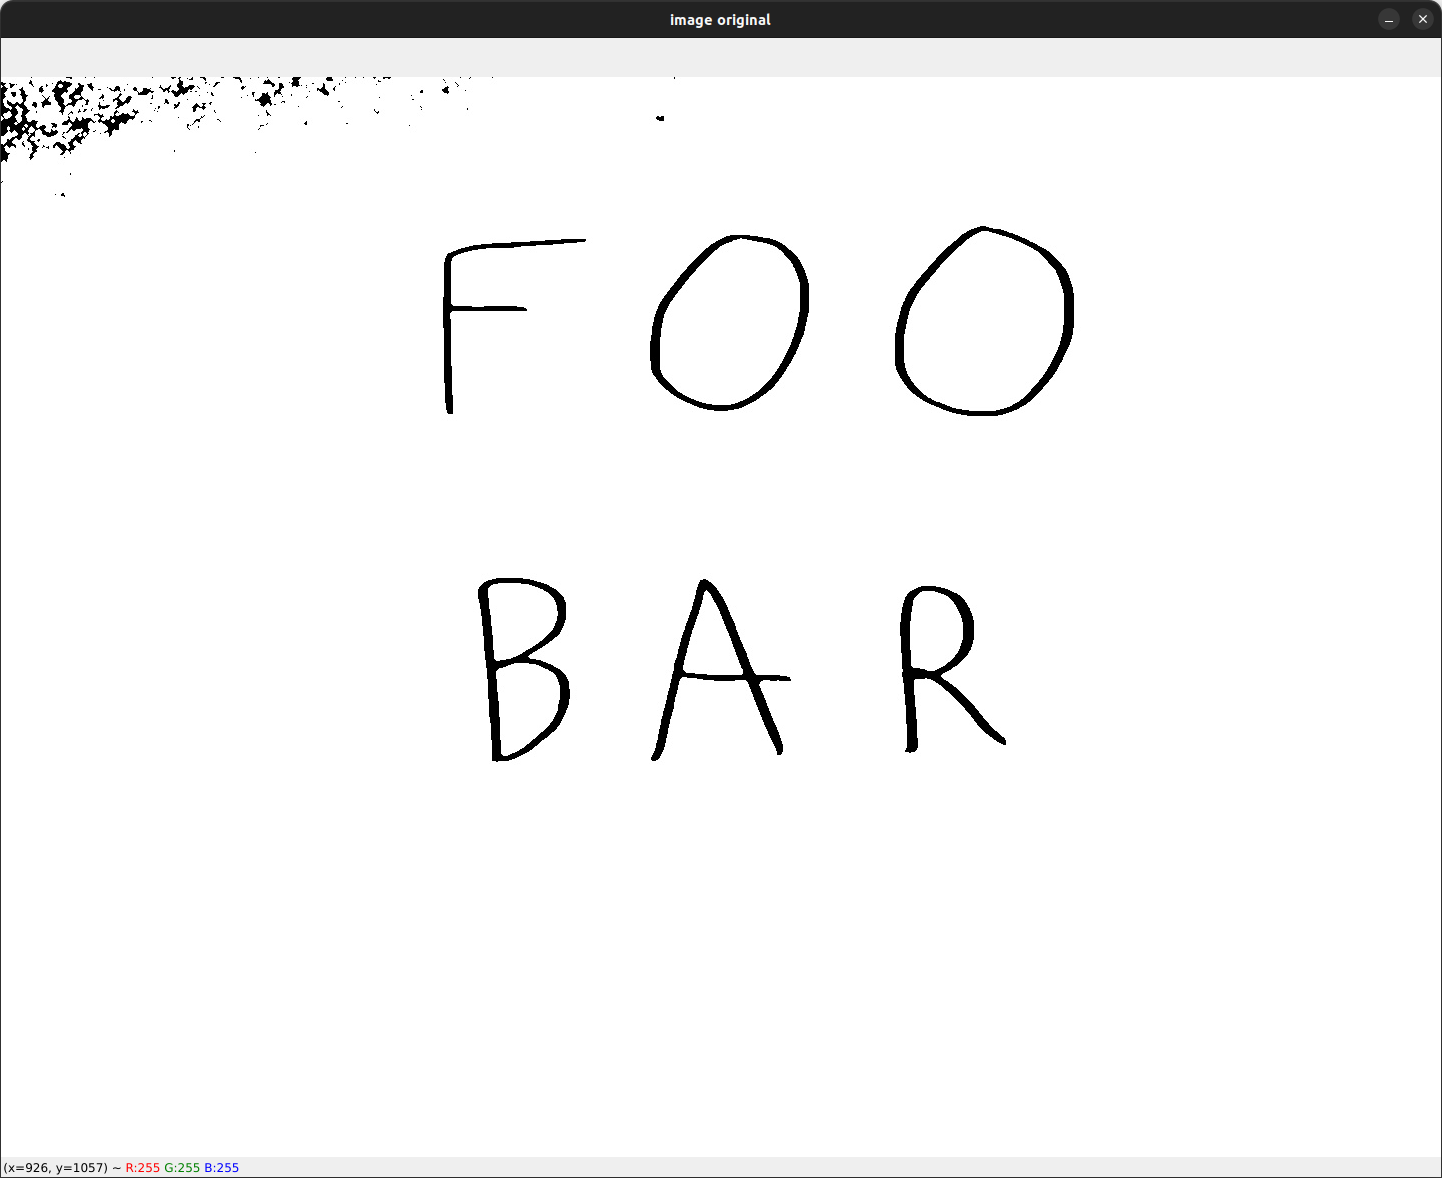
\includegraphics[width=\textwidth]{segmentation_image_originel.png}
				\centering
				\label{fig:imageOriginel}
			\end{figure}
			\paragraph{} Sur la figure \ref{fig:imageOriginel}, nous voyons une image de bonne qualité prête à être segmenter par l'algorithme n°\ref{alg:segmentation} (page\pageref{alg:segmentation}). 
			\begin{figure}
				\caption{Images des deux lignes extraites à partir de l'image de départ}
				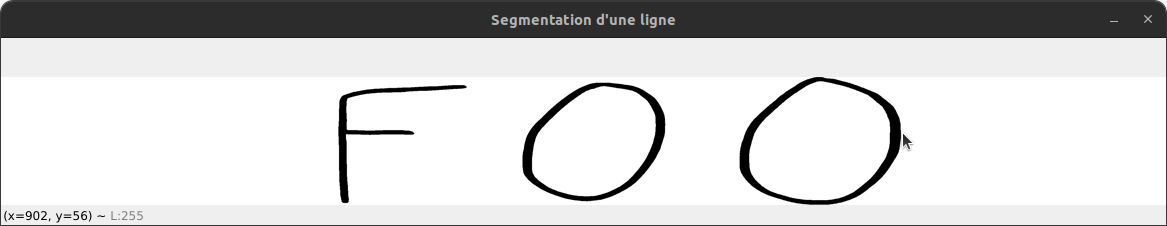
\includegraphics[width=.8\textwidth]{segmentation_ligne1.png}
				\centering
				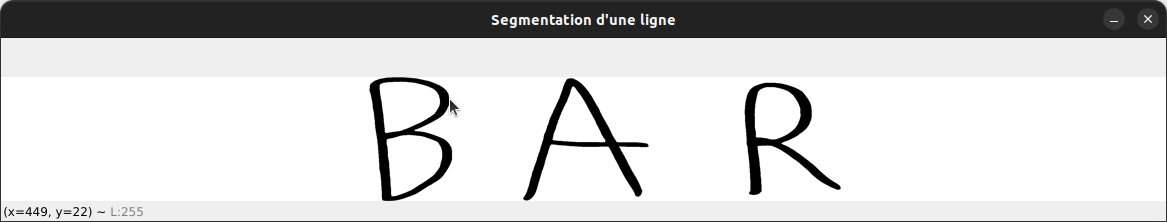
\includegraphics[width=.8\textwidth]{segmentation_ligne2.png}
				\centering
				\label{fig:imageLignes}
			\end{figure}
			% \paragraph{} On voit sur la figure \ref{fig:imageLignes} à la page \pageref{fig:imageLignes} que dû à un filtrage de bonne qualité, nous obtenons exactement 2 lignes comme attendus. 
			\begin{wrapfigure}{r}{0.35\textwidth}
					\caption{Structure de données dans l'algorithme SEGMENTATION}
					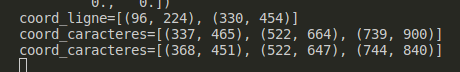
\includegraphics[width=0.35\textwidth]{structDonnee.png}
					\label{fig:structDonnee}
			\end{wrapfigure}
			\paragraph{} Grâce à une projection vertical, nous obtenons ce tableau (figure \ref{fig:structDonnee}). La 1er ligne de ce tableau contient autant de tuples que le nombre de lignes. Chaque tuples contient la composante en ordonnée du début et de la fin d'une ligne. Ensuite, on extrait nos 2 lignes comme sur la figure \ref{fig:imageLignes} depuis l'image d'entrée.
			\paragraph{} Après avoir isolé les lignes, on procède à la séparation des caractères contenus dans chaque lignes en suivant l'algorithme n°\ref{alg:coordcar} page \pageref{alg:coordcar}
			\paragraph{} Étant donné que l'image est binairisée, lorsqu'un carctère est présent à un endroit donné, cela signifie que sur la projection verticale de l'histogramme est supérieur à 0 à cette position. L'algorithme n°\ref{alg:coordcar} va parcourir cette projection de l'histogramme, déctecter les pics et récupérer l'indice de début et de fin de ces derniers qui correspondront à la limite gauche et droit d'un caractère sur l'image. Nous pouvons voir le résultats de cette fonction sur la figure \ref{fig:structDonnee} et des histogrammes de projection horizontal dans l'annexe (page \pageref{fig:histoX1}).
			\begin{figure}
				\caption{Imagettes des caractères créées à partir de la 1e ligne}
				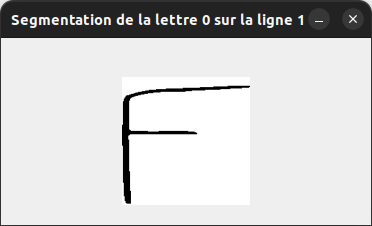
\includegraphics[scale=.3]{segmentation_F.png}
				\centering
				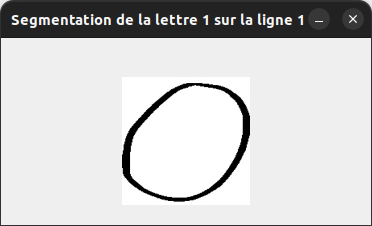
\includegraphics[scale=.3]{segmentation_O1.png}
				\centering
				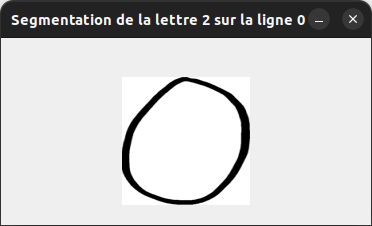
\includegraphics[scale=.3]{segmentation_O2.png}
				\centering
			\end{figure}
			\begin{figure}
				\caption{Imagettes des caractères créées à partir de la 2e ligne}
				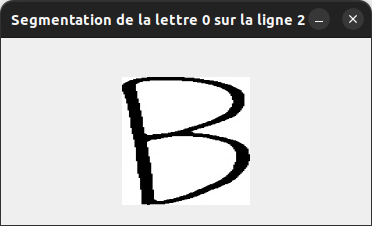
\includegraphics[scale=.3]{segmentation_B.png}
				\centering
				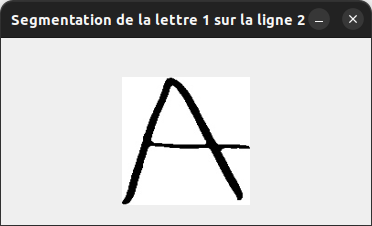
\includegraphics[scale=.3]{segmentation_A.png}
				\centering
				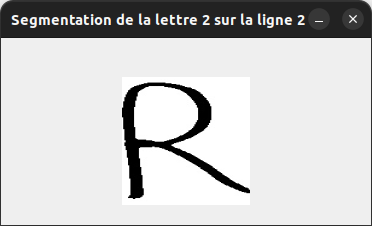
\includegraphics[scale=.3]{segmentation_R.png}
				\centering
			\end{figure}
	\newpage
	\section{Analyse des Résulats}
		\subsection{Mesure expérimental de YOLO}
			Notre procédure de test est la suivante : Écrire une suite de caractère de moins en moins bien écrit pour chaque lettre de l'alphabet, ???, YOLO, grah
			\begin{figure}[H]
				\caption{}
				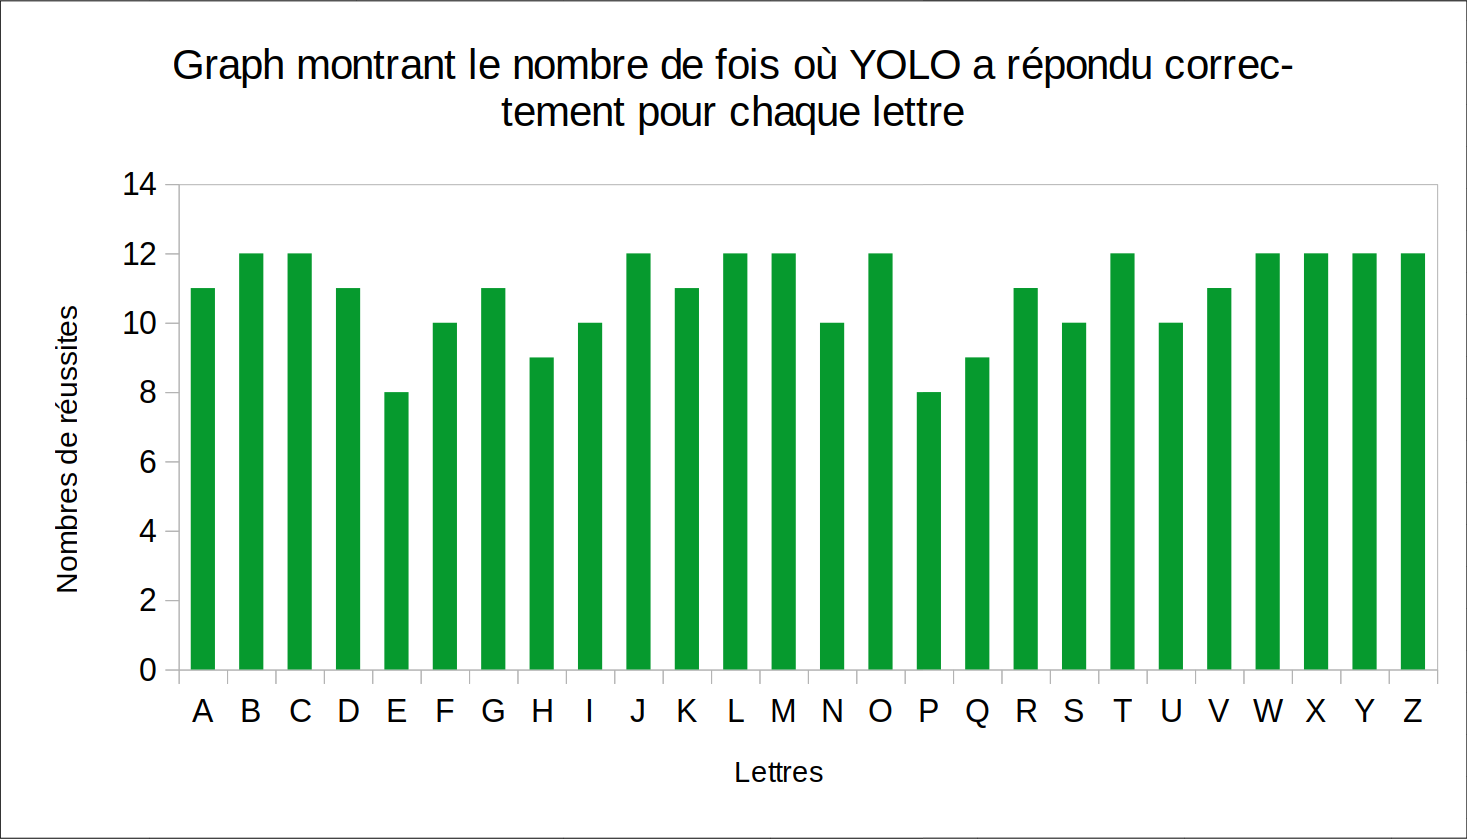
\includegraphics[width=\textwidth]{grapYoloReussite.png}
				\centering
				\label{fig:graph:reussite}
			\end{figure}
			\begin{figure}[H]
				\caption{}
				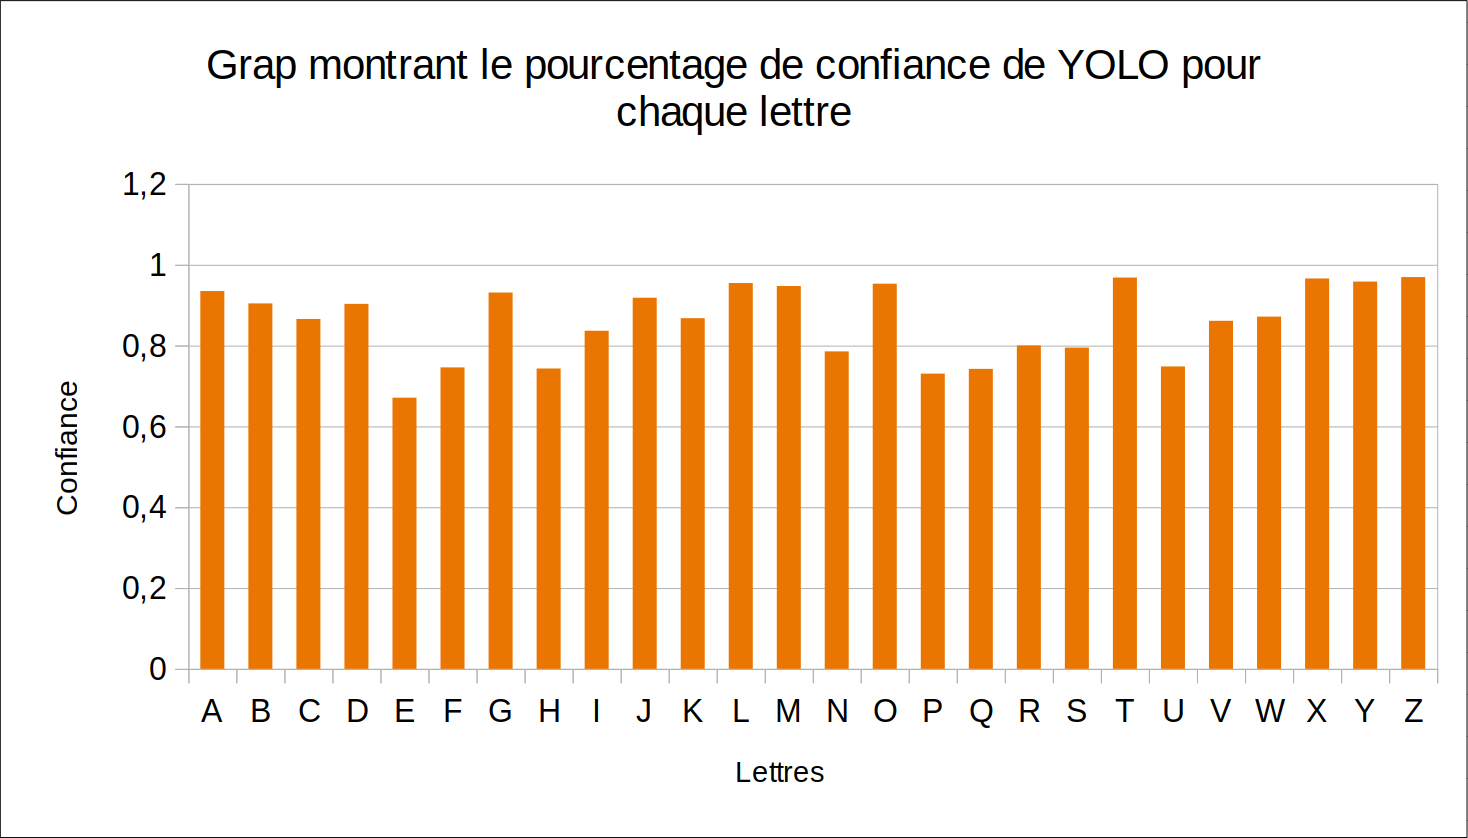
\includegraphics[width=\textwidth]{grapYoloConfiance.png}
				\centering
				\label{fig:graph:confiance}
			\end{figure}
	\section{Gestion du Projet}
		\paragraph{} Pendant ce projet, nous avions dû communiquer régulièrement afin d'être au point sur les éléments à développer ou corriger, nécessitant ainsi l'utilisation de Discord.
		\paragraph{} De plus, pour le partage de code et le versioning, nous avions utilisés git et Github
		Laurent : filtrage, segmentation
		Romain : IHM, YOLO
		Tony : rapport, segmentation 
	\addcontentsline{toc}{section}{Bilan et Conclusions}%insert dans le toc
	\section*{Bilan et Conclusions}%sans numéro et pas dans le toc
		\paragraph{}
			tests
		\paragraph{}
			Cependant, certains points laissent à désirer dans notre projet. Malheureusement, une contribution de l'utilisateur est nécessaire. Pour une bonne reconnaissance des caractères, l'utilisateur doit rogner l'image. Il serait plus pratique que le \emph{rognagne soit fait automatiquement}. 
		\paragraph{}
			Ensuite, au niveau de la \emph{segmentation}, notre algorithme n'est pas capable de séparer des lettre cursives et ignore totalement les espaces.
		\paragraph{}
			Et enfin, dans le futur, le but sera que \emph{YOLO} reconnaisse aussi l'alphabet minuscule mais aussi l'alphabet français (avec les accents).
%		meilleur segmentation : segmentation des lettres cursives, reconnaissance des espaces
%		modifier les hyper paramètres de yolo
%		YOLO : lettres minuscule, avec accents
	\newpage
	\section*{Bibliographie}
		% \bibliographystyle{plain} % We choose the "plain" reference style
		% \bibliography{refs} % Entries are in the refs.bib file
	\newpage
	\section*{Annexes}
		\begin{figure}[H]
			\caption{Histogramme de projection vertical}
			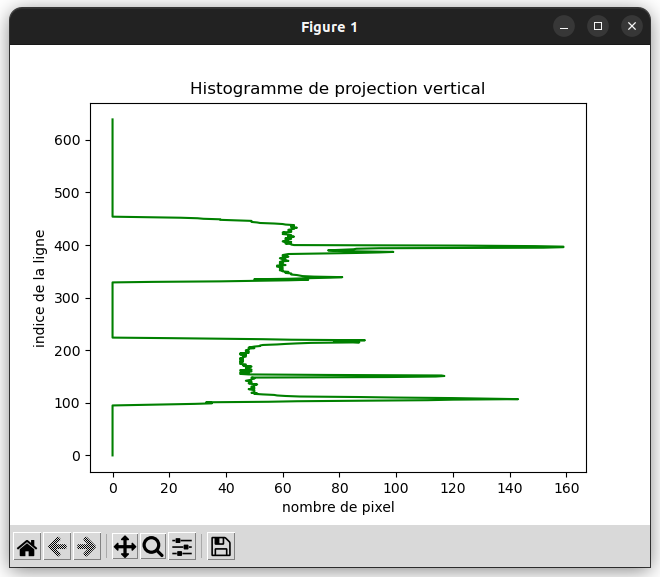
\includegraphics[width=.7\textwidth]{histoY.png}
			\centering
			\label{fig:histoY}
		\end{figure}
		\begin{figure}[H]
			\caption{Histogramme de projection horizontal}
			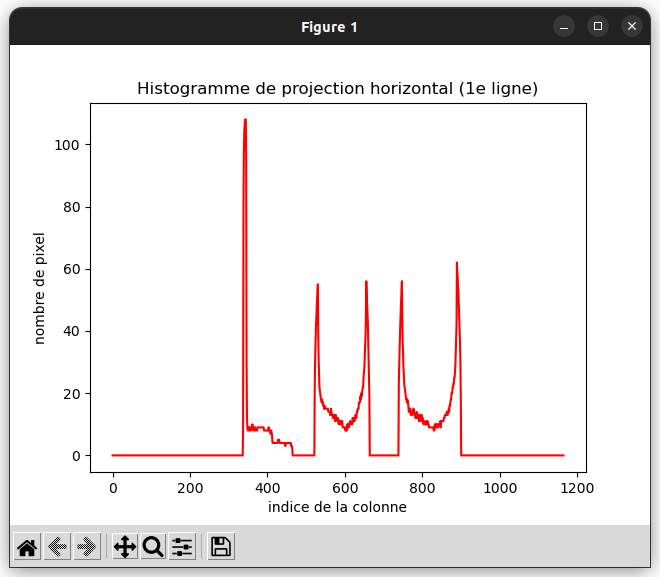
\includegraphics[width=0.7\textwidth]{histoX1.png}
			\centering
			\label{fig:histoX1}
		\end{figure}
		\begin{figure}[H]
			\caption{Histogramme de projection horizontal}
			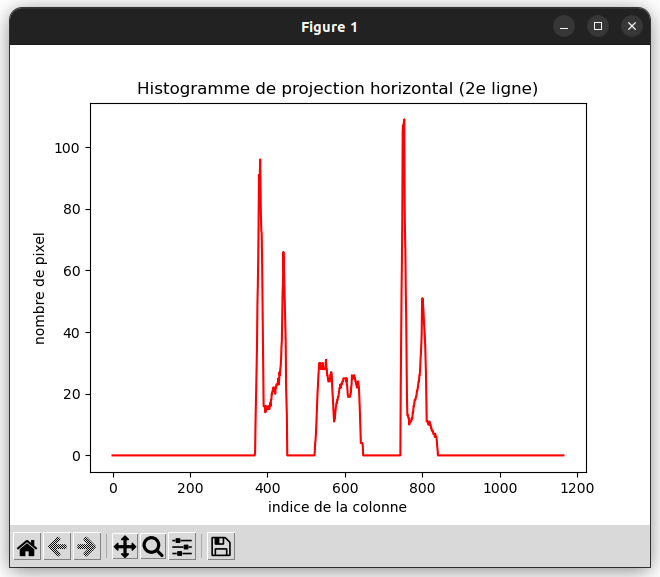
\includegraphics[width=.7\textwidth]{histoX2.png}
			\centering
			\label{fig:histoX2}
		\end{figure}
\end{document}